\documentclass[../../main.tex]{subfiles}
\begin{document}

\begin{flushright}
\footnotesize\textit{【自動文字起こし・要確認】}
\end{flushright}

{\bf [解]}
\textbf{(1)} $a,b>0$とし$g(t)=\dfrac1bt^a-\log t$（$t>0$）とおく．
\begin{align*}
g'(t)=\frac abt^{a-1}-\frac1t=\frac1t\Bigl(\frac abt^a-1\Bigr)
\end{align*}
より，$g'(t)=0\iff t=\bigl(\frac ba\bigr)^{\frac1a}$．この点の前後で$g'$は$-$から$+$に変わるので，$g$は$t=\bigl(\frac ba\bigr)^{1/a}$で極小値
\begin{align*}
g\Bigl(\Bigl(\frac ba\Bigr)^{\frac1a}\Bigr)=\frac1a-\frac1a\log\frac ba
\end{align*}
をとる（$t\to0^+,\,t\to\infty$でともに$g(t)\to+\infty$なのでこれは最小値でもある）．

\textbf{(2)} $m>0$とする．条件(b)は$t>0$すべてで成り立つ不等式なので，(1)の結果を$a=x,\ b=y$として用いて言い換える．$g(t)=\frac1yt^x-\log t$の最小値は$t=(y/x)^{1/x}$で$\frac1x\bigl(1-\log\frac yx\bigr)$だから，条件(b)は
\begin{align*}
\frac1x\Bigl(1-\log\frac yx\Bigr)\ge m
\end{align*}
と同値．$x>0$に注意して整理すると$\log\dfrac yx\le1-mx$，すなわち
\begin{align*}
y\le x\cdot e^{1-mx}\equiv f(x)
\end{align*}
となる．よって$D$は
\begin{align*}
0<x<y\le f(x)=x\,e^{1-mx}
\end{align*}
で定まる領域である．
\begin{align*}
f'(x)=e^{1-mx}(1-mx)
\end{align*}
より$f$は$x=\frac1m$で最大値$f(\frac1m)=\frac1m$をとり，$x\to0^+$と$x\to\infty$でともに$f(x)\to0$．また
\begin{align*}
f(x)\ge x\iff e^{1-mx}\ge1\iff x\le\frac1m
\end{align*}
（$x>0$より）．したがって$0<x\le\frac1m$では直線$y=x$と曲線$y=f(x)$の間（$x<y\le f(x)$）が存在し，$x>\frac1m$では$f(x)<x$となるので$D$は空である．よって$D$は図の斜線部分（境界は太線部を含み，点線部および$x=0$は含まない）．

\begin{figure}[htb]
\centering
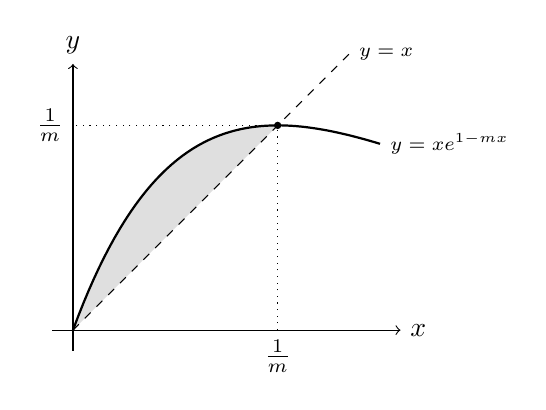
\begin{tikzpicture}[scale=2.6]
  \draw[->] (-0.1,0) -- (1.6,0) node[right]{$x$};
  \draw[->] (0,-0.1) -- (0,1.3) node[above]{$y$};
  \fill[gray!25] plot[domain=0:1,samples=40] (\x,{\x*exp(1-\x)}) -- (0,0) -- cycle;
  \draw[dashed] (0,0) -- (1.35,1.35) node[right]{\scriptsize$y=x$};
  \draw[thick,domain=0:1.5,samples=60] plot (\x,{\x*exp(1-\x)}) node[right]{\scriptsize$y=xe^{1-mx}$};
  \draw[dotted] (1,0) -- (1,1) -- (0,1);
  \node[below] at (1,0) {$\frac1m$};
  \node[left] at (0,1) {$\frac1m$};
  \filldraw (1,1) circle(0.015);
\end{tikzpicture}
\caption{領域$D$（斜線部，$m=1$の場合の概形）}
\end{figure}

\textbf{(3)} 面積$S$は
\begin{align*}
S=\int_0^{\frac1m}\bigl(x\,e^{1-mx}-x\bigr)\,dx=e\int_0^{\frac1m}x\,e^{-mx}\,dx-\frac12\Bigl(\frac1m\Bigr)^2
\end{align*}
部分積分により$\displaystyle\int xe^{-mx}\,dx=-e^{-mx}\Bigl(\frac xm+\frac1{m^2}\Bigr)+C$なので
\begin{align*}
\int_0^{\frac1m}xe^{-mx}\,dx=\Bigl[-e^{-mx}\Bigl(\frac xm+\frac1{m^2}\Bigr)\Bigr]_0^{\frac1m}=-e^{-1}\cdot\frac2{m^2}+\frac1{m^2}=\frac1{m^2}\Bigl(1-\frac2e\Bigr)
\end{align*}
ゆえに
\begin{align*}
S=e\cdot\frac1{m^2}\Bigl(1-\frac2e\Bigr)-\frac1{2m^2}=\frac{e-2}{m^2}-\frac1{2m^2}=\Bigl(e-\frac52\Bigr)\frac1{m^2}
\end{align*}


\newpage

\end{document}
